\section{Speckle y procesamiento}

\subsection{Ecuación de radar}
\begin{frame}{\secname : \subsecname}
    \begin{block}{Definición}
      \begin{equation}
        P_r = \frac{P_t G_t G_r \lambda^2 \sigma}{(4\pi)^3 R^4}
      \end{equation}
      Con $P_r$ y $P_t$ las las potencias recibidas y transmitidas, $G_r$ y $G_t$ las ganancias del emisor y receptor, $\lambda$ la longitud de onda, $\sigma$ el coeficiente de backscatter y $R$ la distancia entre el emisor y el blanco.
    \end{block}
\end{frame}
%--- Next Frame ---%

\subsection{decibels}
\begin{frame}{\secname : \subsecname}
    \begin{block}{Definición}
      Es común expresar la potencia de un radar en decibels cómo
      \begin{equation}
        P [dB] = 10\log_{10}(P_r)
      \end{equation}
      donde $P_r$ es una potencia reflejada.
    \end{block}
\end{frame}
%--- Next Frame ---%

\subsection{Speckle}
\begin{frame}{\secname : \subsecname}
  \begin{figure}
    \centering
    \movie[width = 0.95\textwidth,loop,autostart]{\centering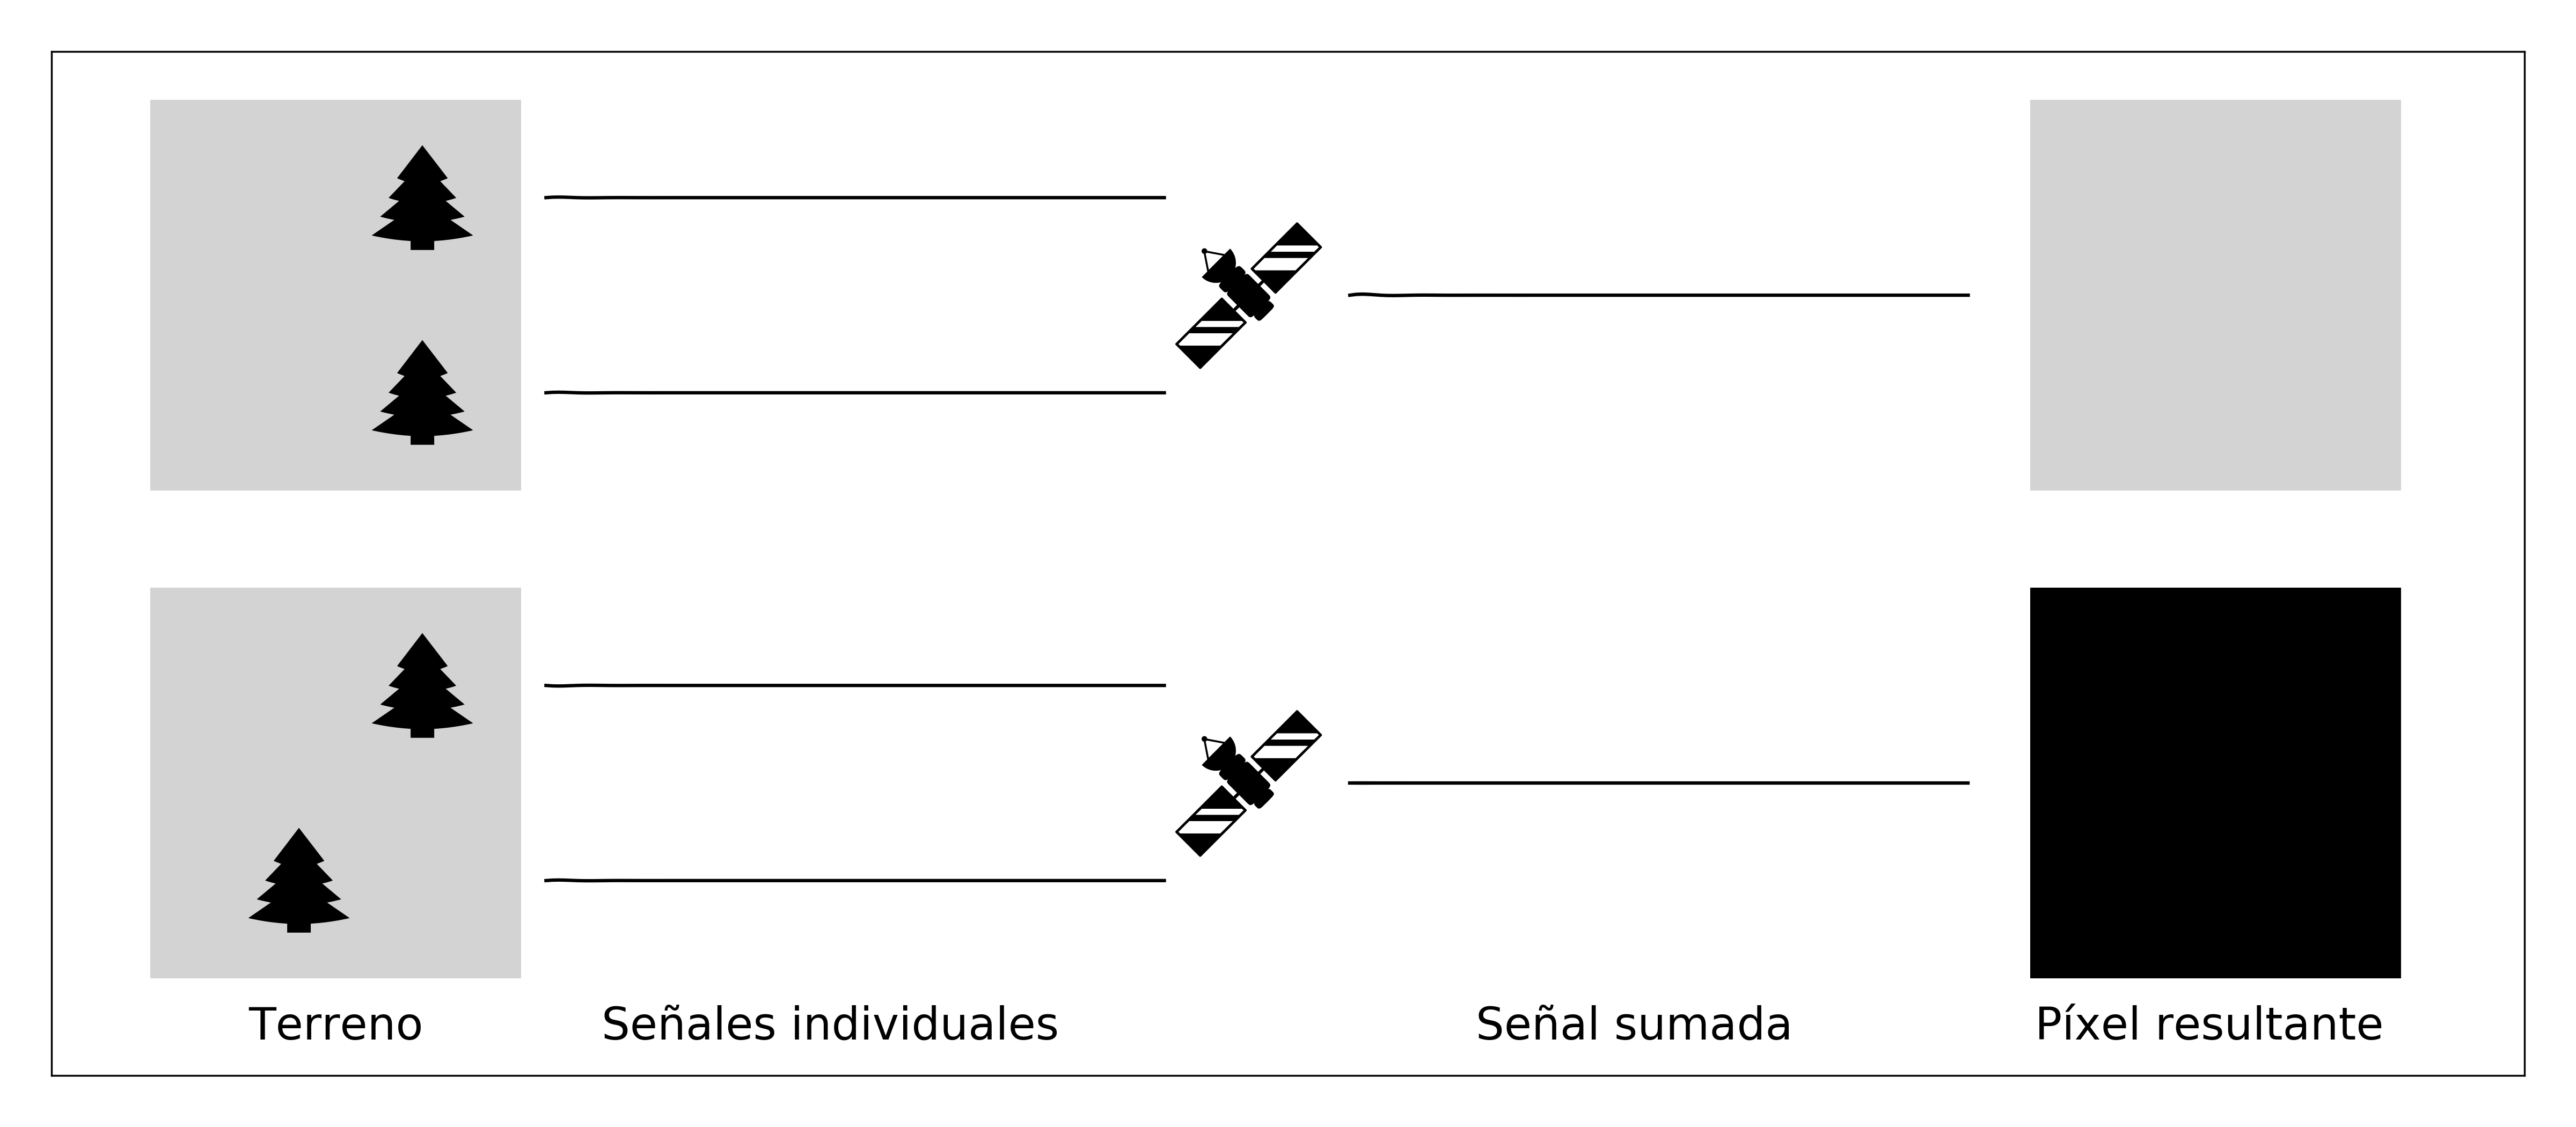
\includegraphics[width=0.95\textwidth]{fig:speckle.png}}{./figs/fig:speckle.mp4}
    \caption{ }
    \label{}
  \end{figure}
\end{frame}
%--- Next Frame ---%

\begin{frame}{\secname : \subsecname}
  \begin{itemize}
    \item El radar suma su señal de manera compleja, modulo y fase.
    \item Como todos los blancos no están en fase la suma no es siempre constructiva.
    \item El specke no es ruido en el sentido que es determinístico. Si repito la adquisición manteniendo la geometría el patrón de specke resulta idéntico.
    \item Si promedio dos pixeles continuos va a volver a pasar lo mismo. Salvo que lo haga en potencia (multilooking)
  \end{itemize}
\end{frame}
%--- Next Frame ---%
\subsection{Reducción de speckle y ruido}
\begin{frame}{\secname : \subsecname}
      \begin{figure}
        \centering
        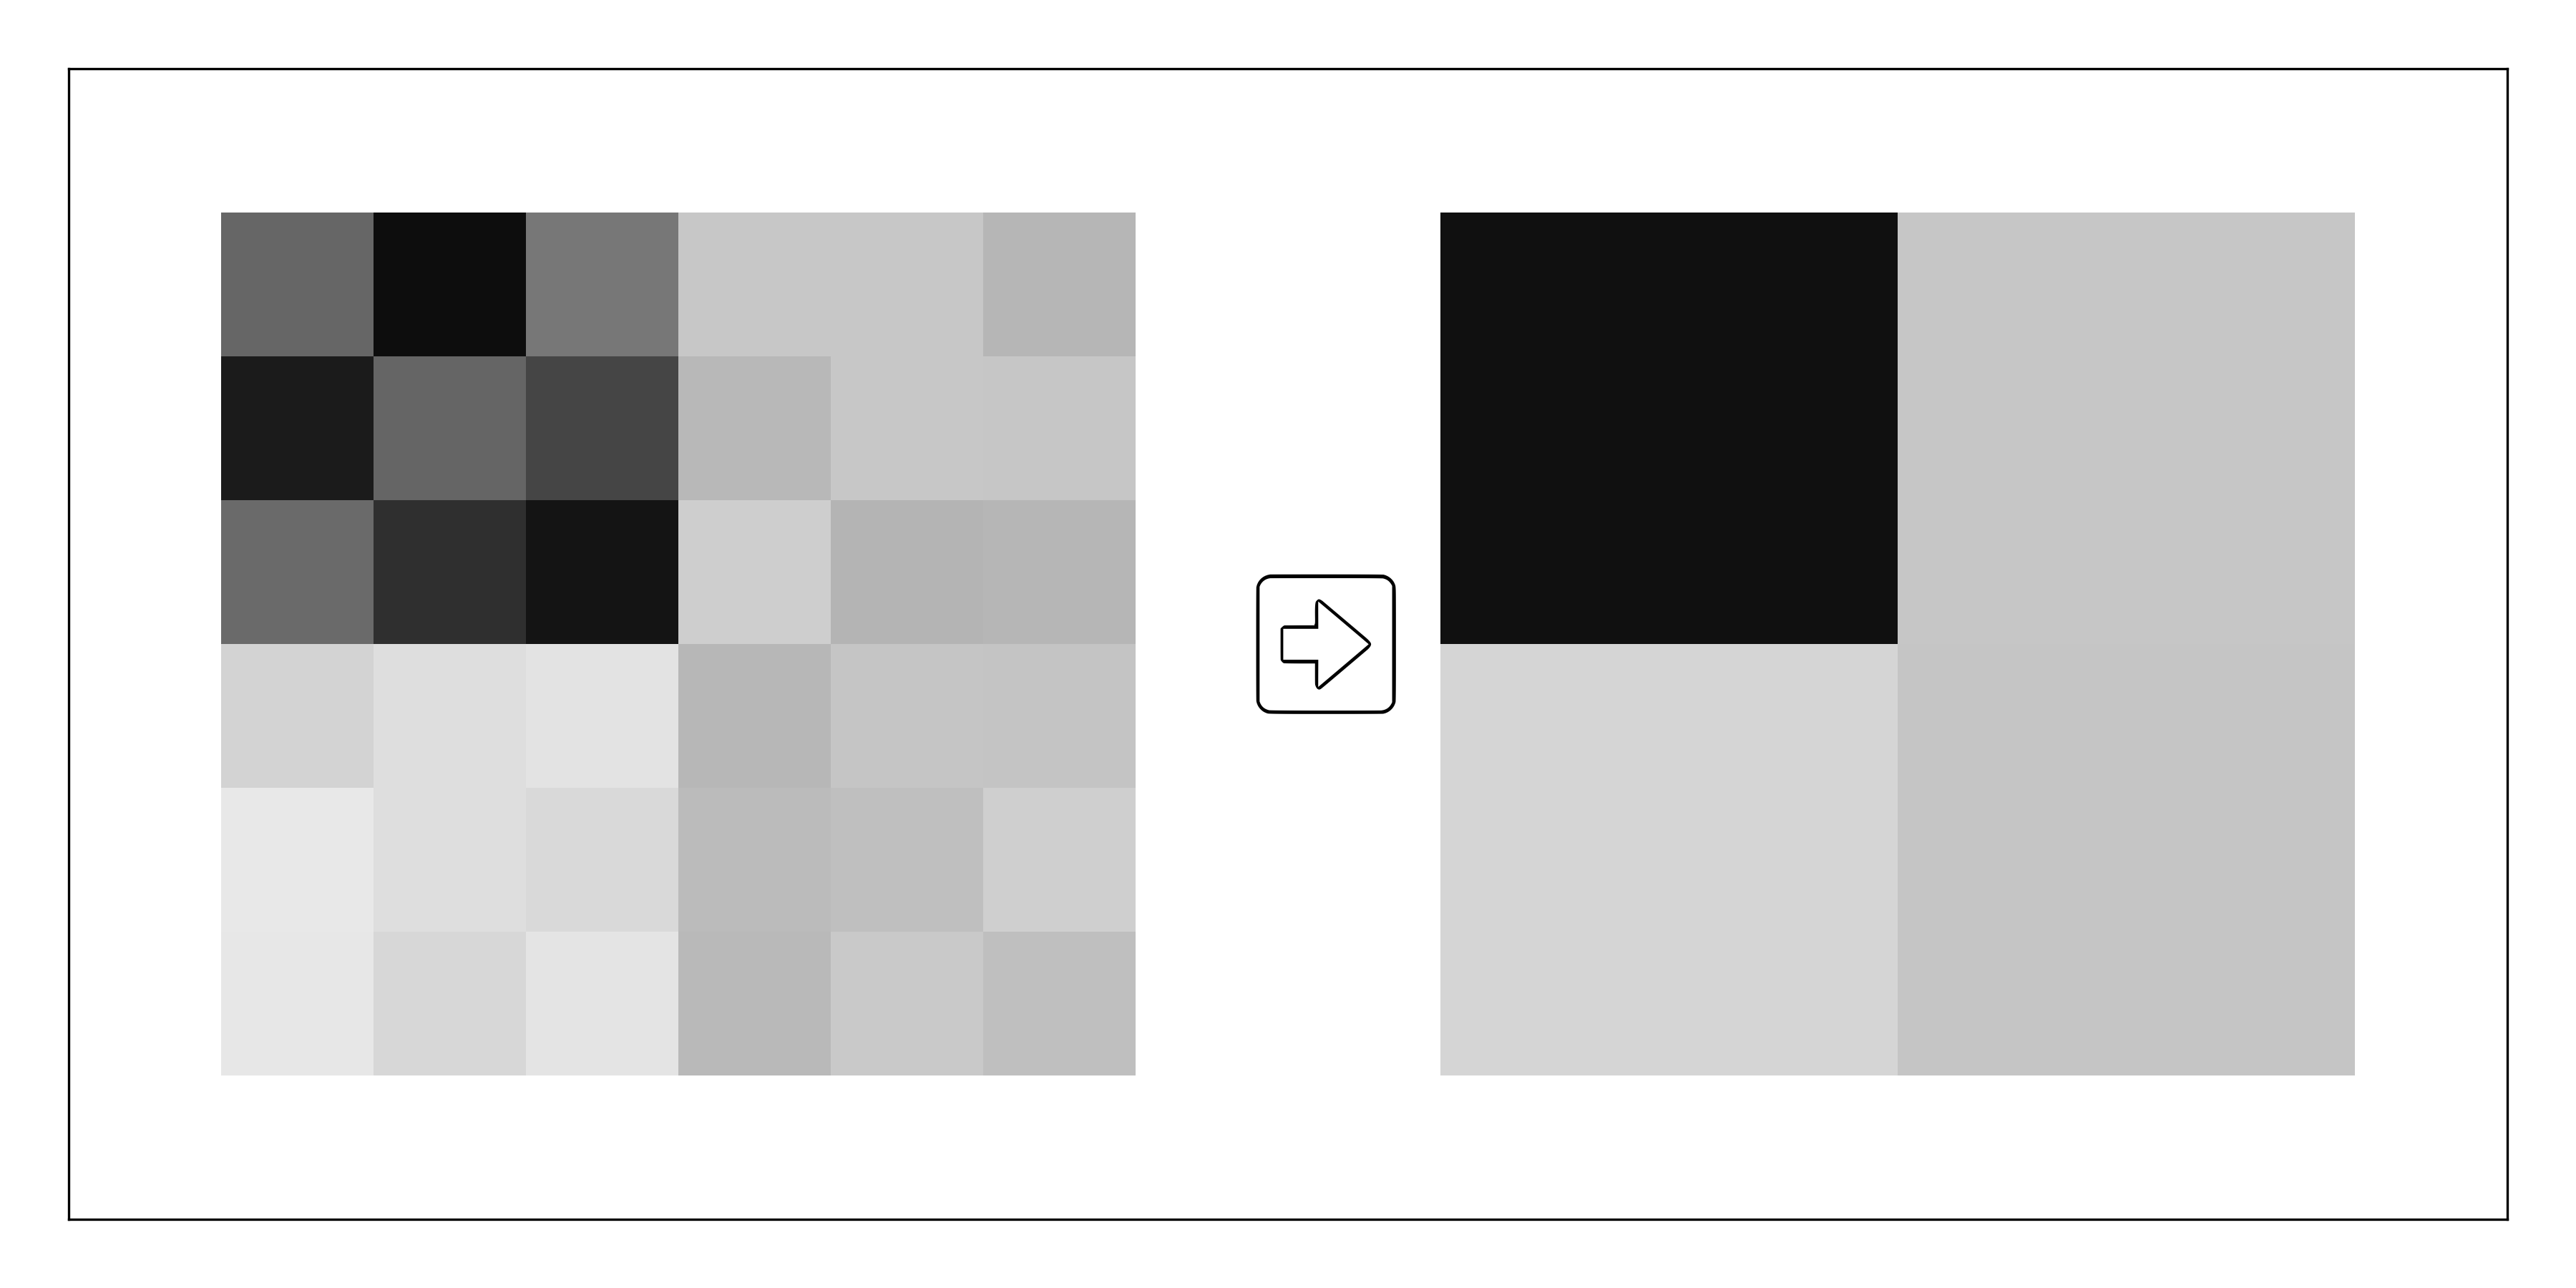
\includegraphics[width=0.9\textwidth]{fig:multilook.png}
        \caption{Proceso de multilook.}
        \label{}
      \end{figure}
\end{frame}
%--- Next Frame ---%

\subsection{Reducción de speckle y ruido}
\begin{frame}{\secname : \subsecname}

   \begin{block}{Multilook}
     \begin{itemize}
       \item Se promedian en potencia varios píxeles vecinos y se los asigna a uno nuevo
       \item Se pierde resolución.
       \item Efectivo contra el speckle.
     \end{itemize}
   \end{block}

\end{frame}
%--- Next Frame ---%

\begin{frame}{\secname : \subsecname}
  \begin{columns}
  \begin{column}{0.5\textwidth}
    \begin{figure}
      \centering
      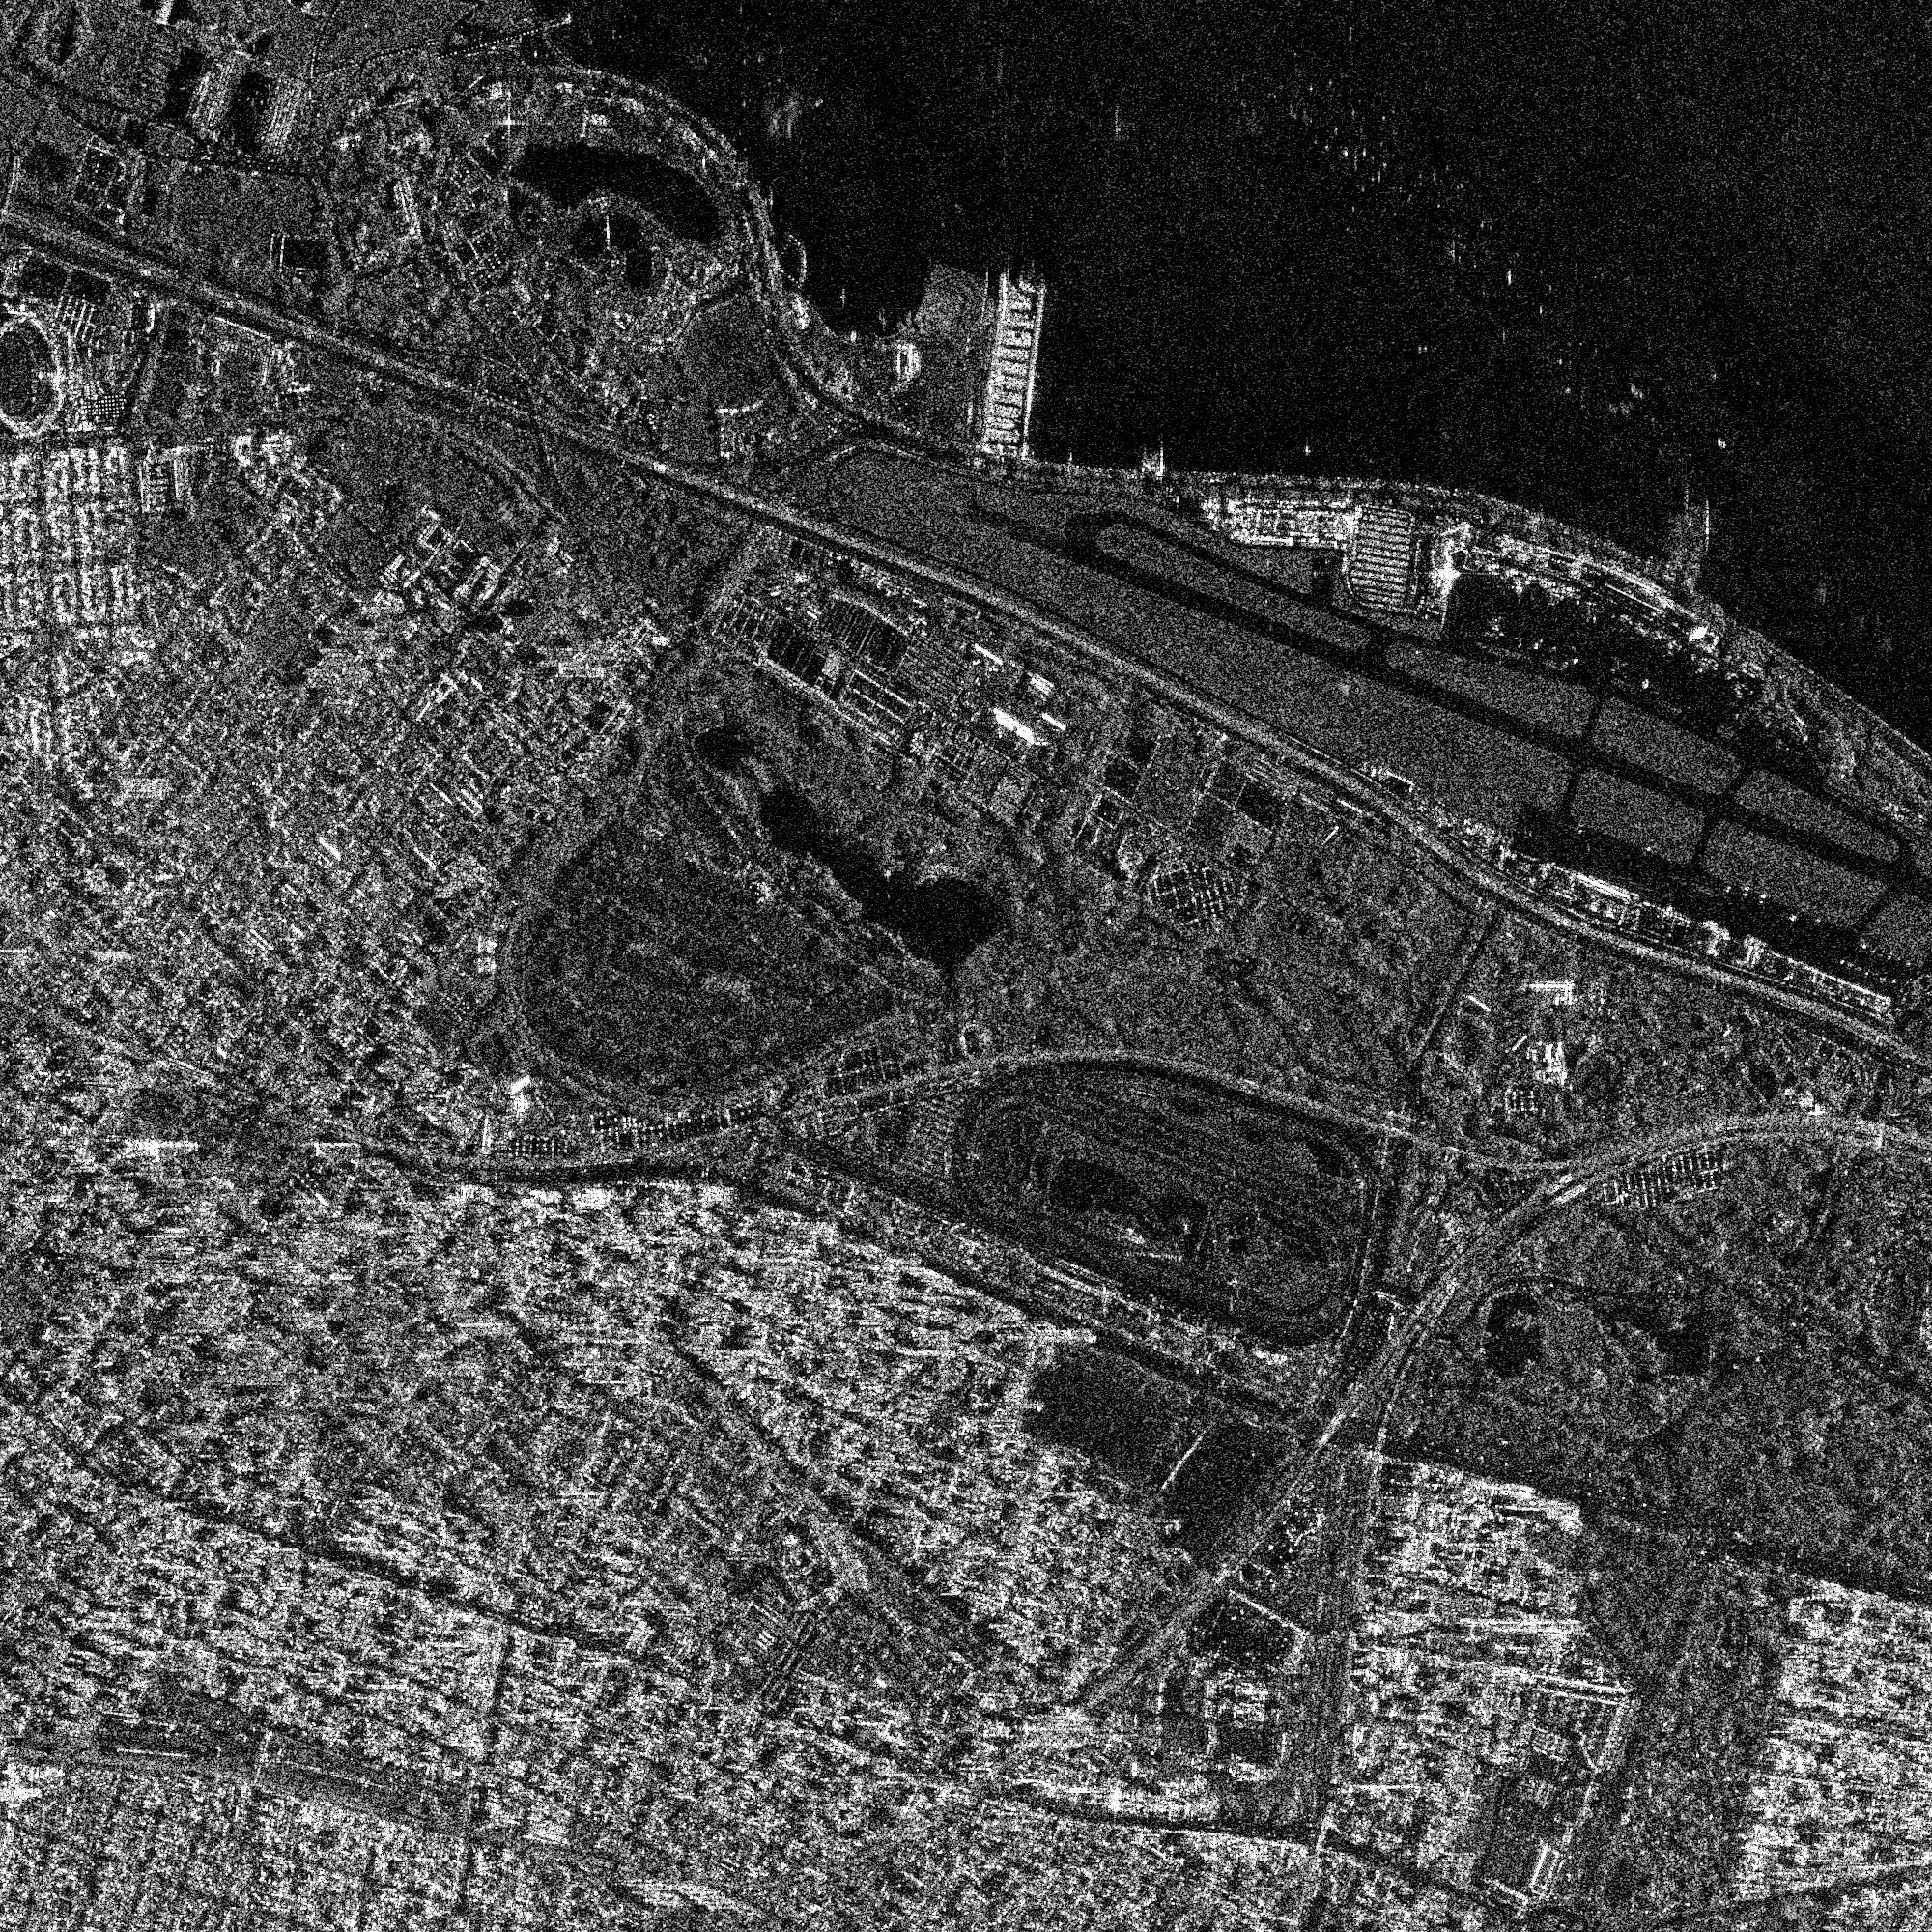
\includegraphics[width=0.8\textwidth]{fig:original.jpg}
      \caption{Imagen original.}
      \label{}
    \end{figure}
  \end{column}
  \begin{column}{0.5\textwidth}  %%<--- here
    \begin{figure}
      \centering
      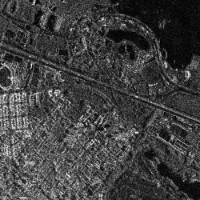
\includegraphics[width=0.8\textwidth]{fig:multilook.jpg}
      \caption{Imagen multilookeada.}
      \label{}
    \end{figure}
  \end{column}
  \end{columns}
\end{frame}
%--- Next Frame ---%


\subsection{Distorciones geométricas}

\begin{frame}{\secname : \subsecname}
  \begin{columns}[t]
    \begin{column}{0.5\textwidth}
      \begin{figure}
        \centering
        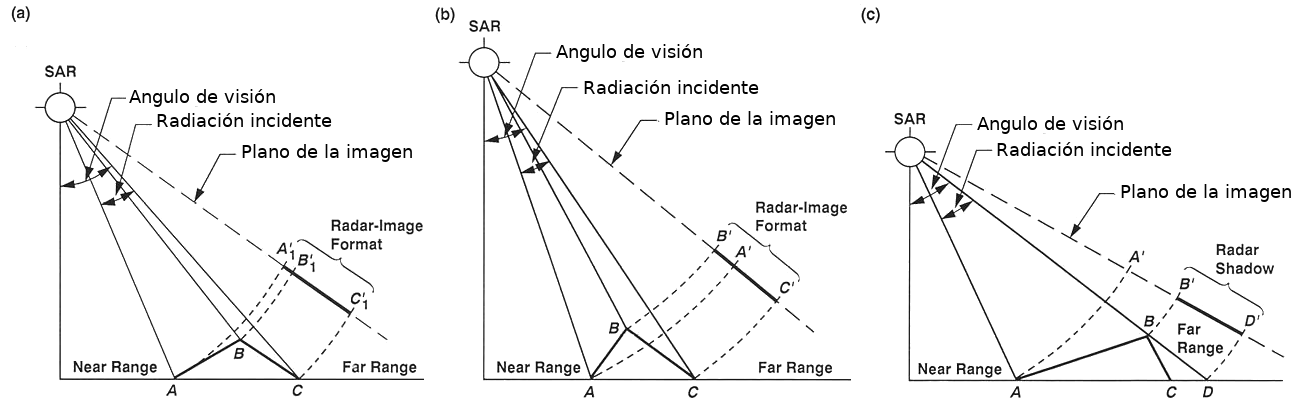
\includegraphics[width=\textwidth]{fig:dist.png}
        \caption{}
        \label{}
      \end{figure}
    \end{column}
    \begin{column}{0.5\textwidth}  %%<--- here
        \begin{figure}
          \centering
          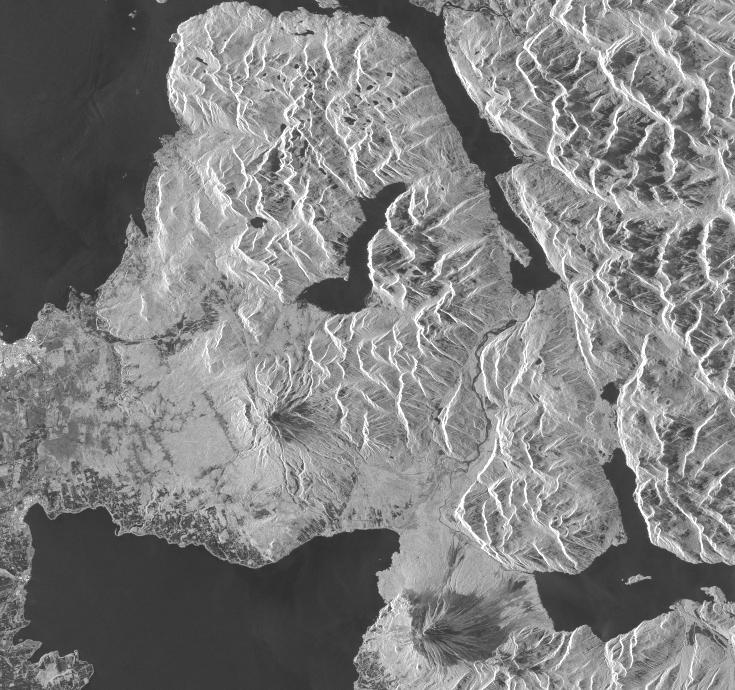
\includegraphics[width=\textwidth]{fig:dist2.jpg}
          \caption{}
          \label{}
        \end{figure}
    \end{column}
    \end{columns}
\end{frame}
%--- Next Frame ---%

\begin{frame}{\secname : \subsecname}
    \begin{figure}
      \centering
      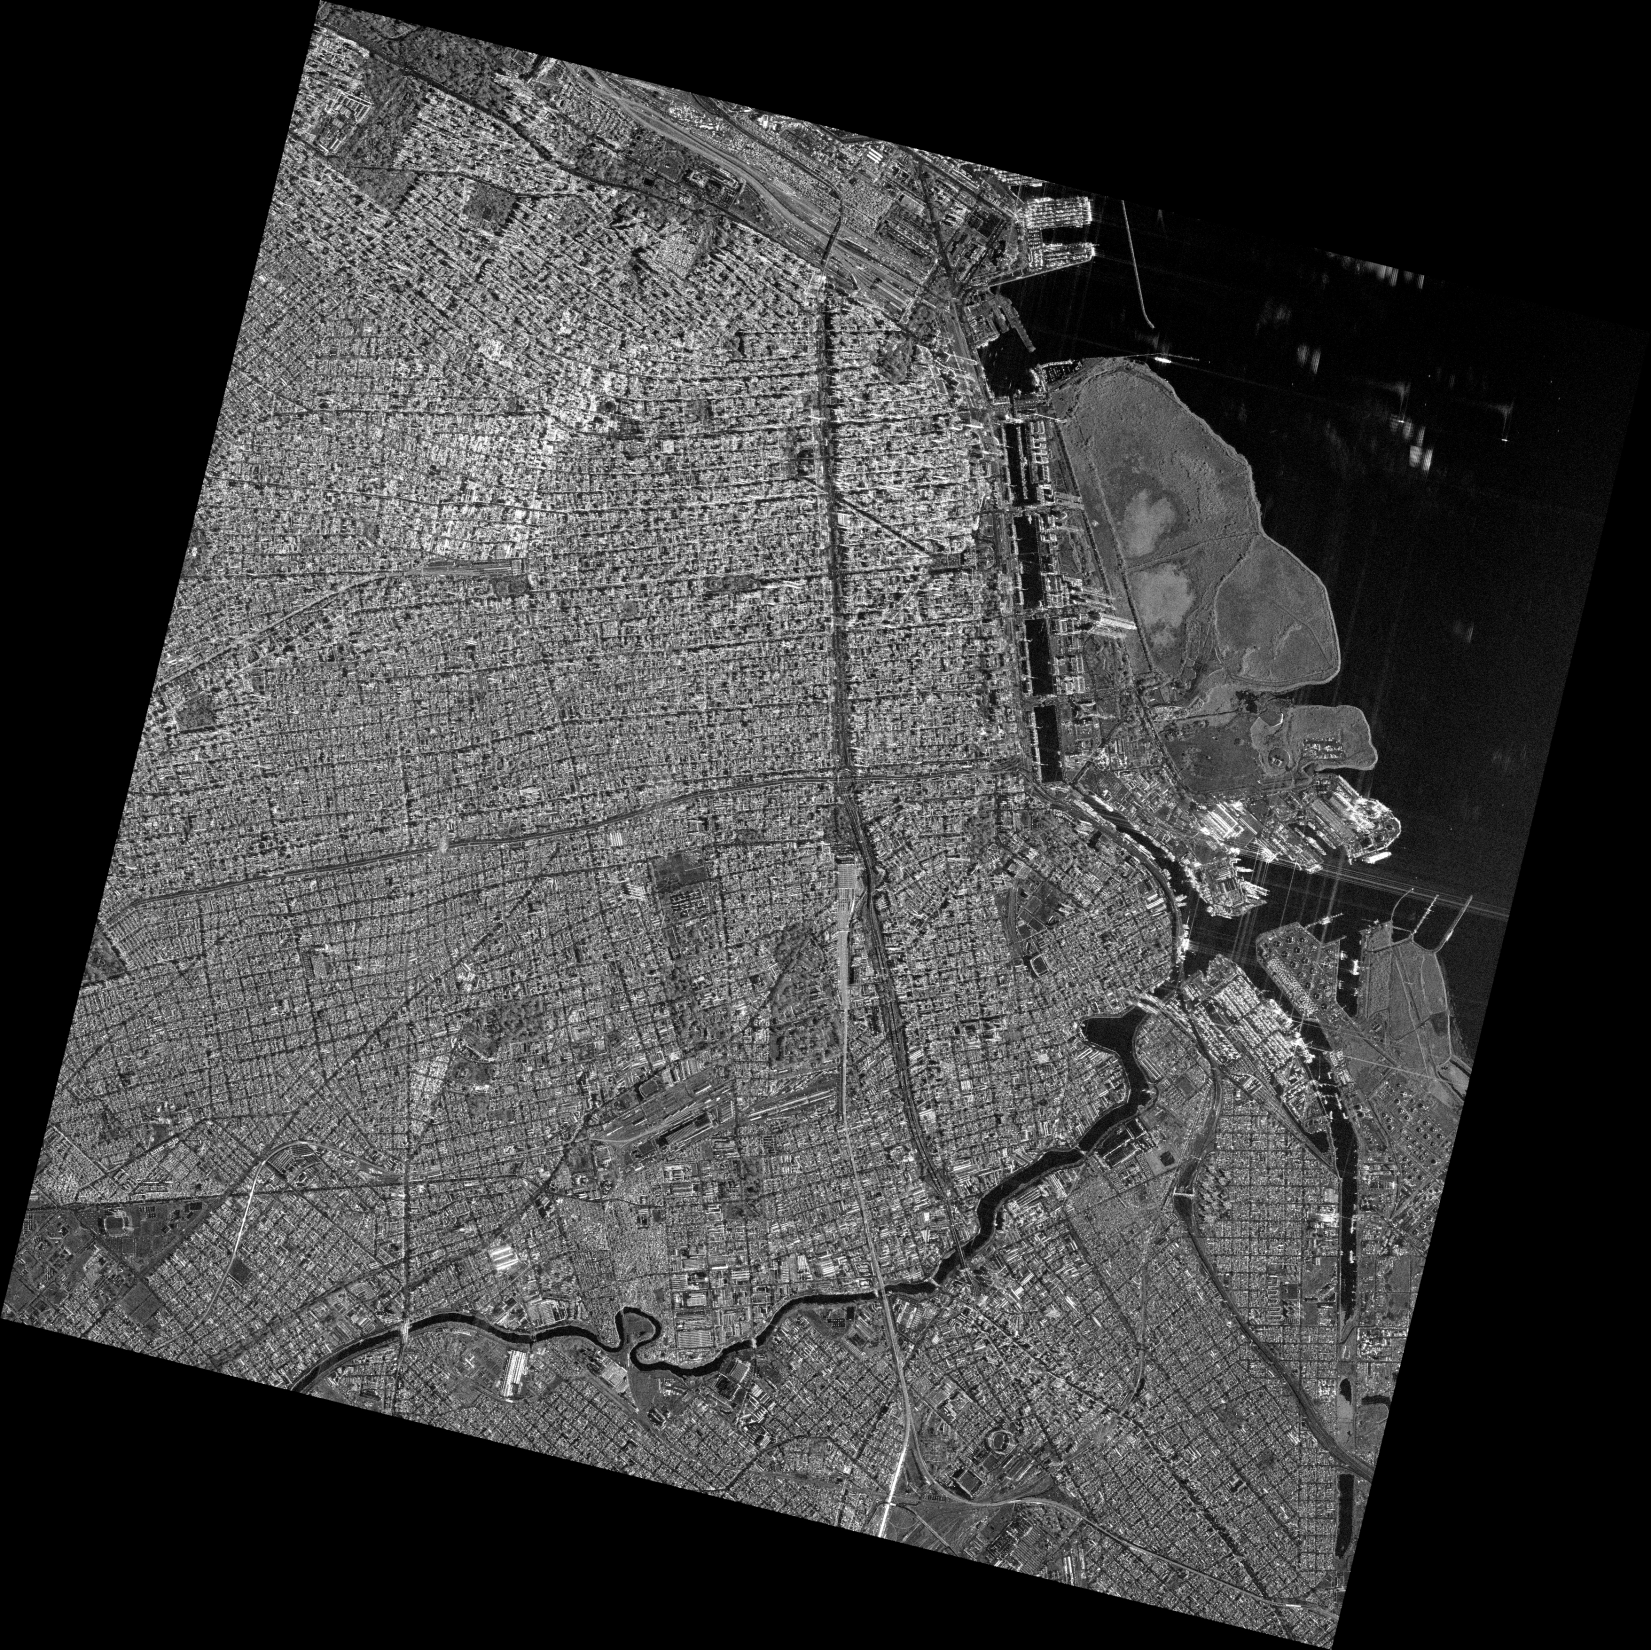
\includegraphics[width=0.5\textwidth]{fig:ba.png}
      \caption{}
      \label{}
    \end{figure}
\end{frame}
%--- Next Frame ---%

\begin{frame}{\secname : \subsecname}
  \begin{columns}[t]
    \begin{column}{0.5\textwidth}
      \begin{figure}
        \centering
        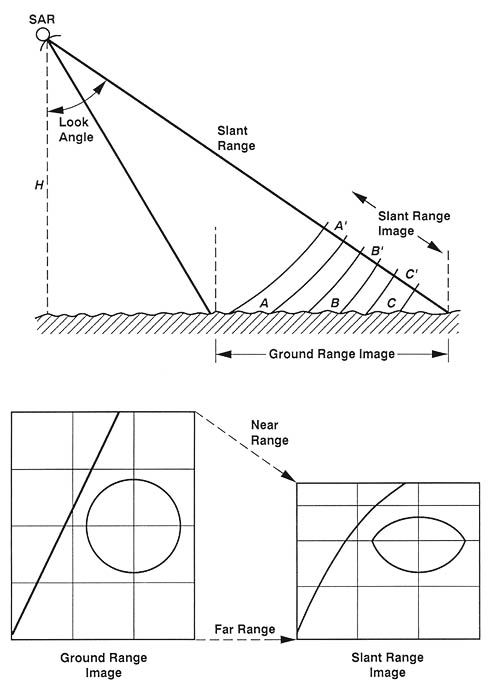
\includegraphics[height=0.7\textheight]{fig:slantground.png}
        \caption{}
        \label{}
      \end{figure}
    \end{column}
    \begin{column}{0.5\textwidth}  %%<--- here
        \begin{figure}

          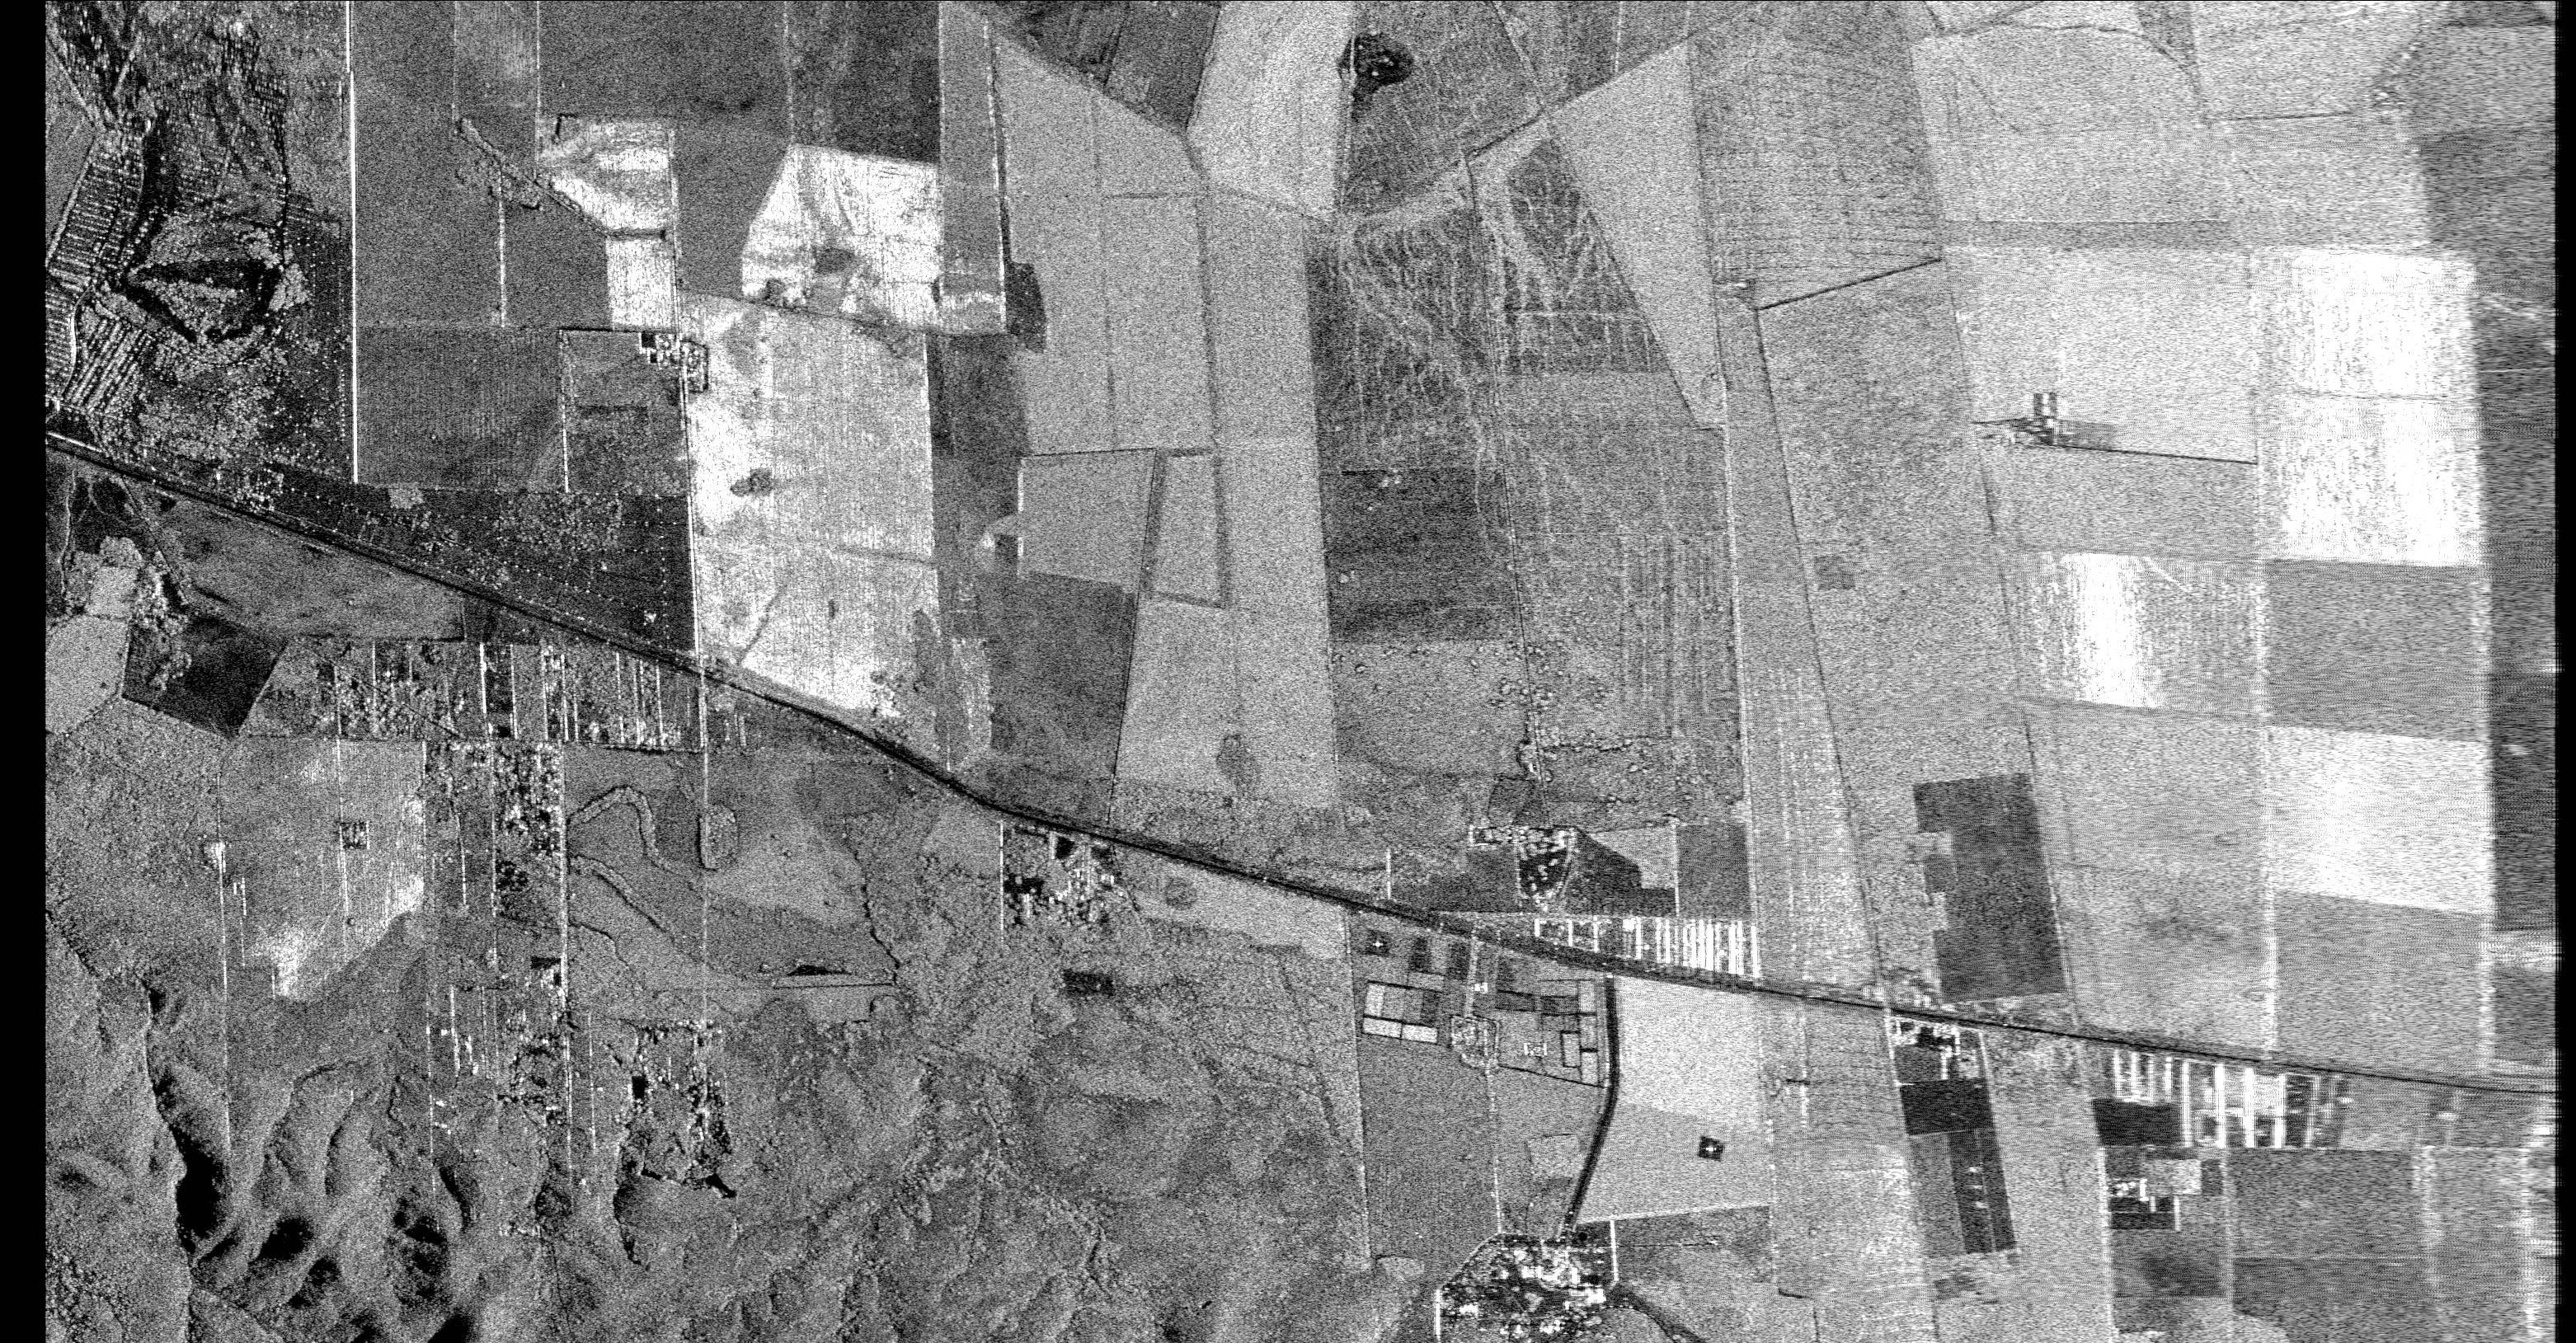
\includegraphics[height=0.2\textwidth]{fig:slant.jpg}\\
          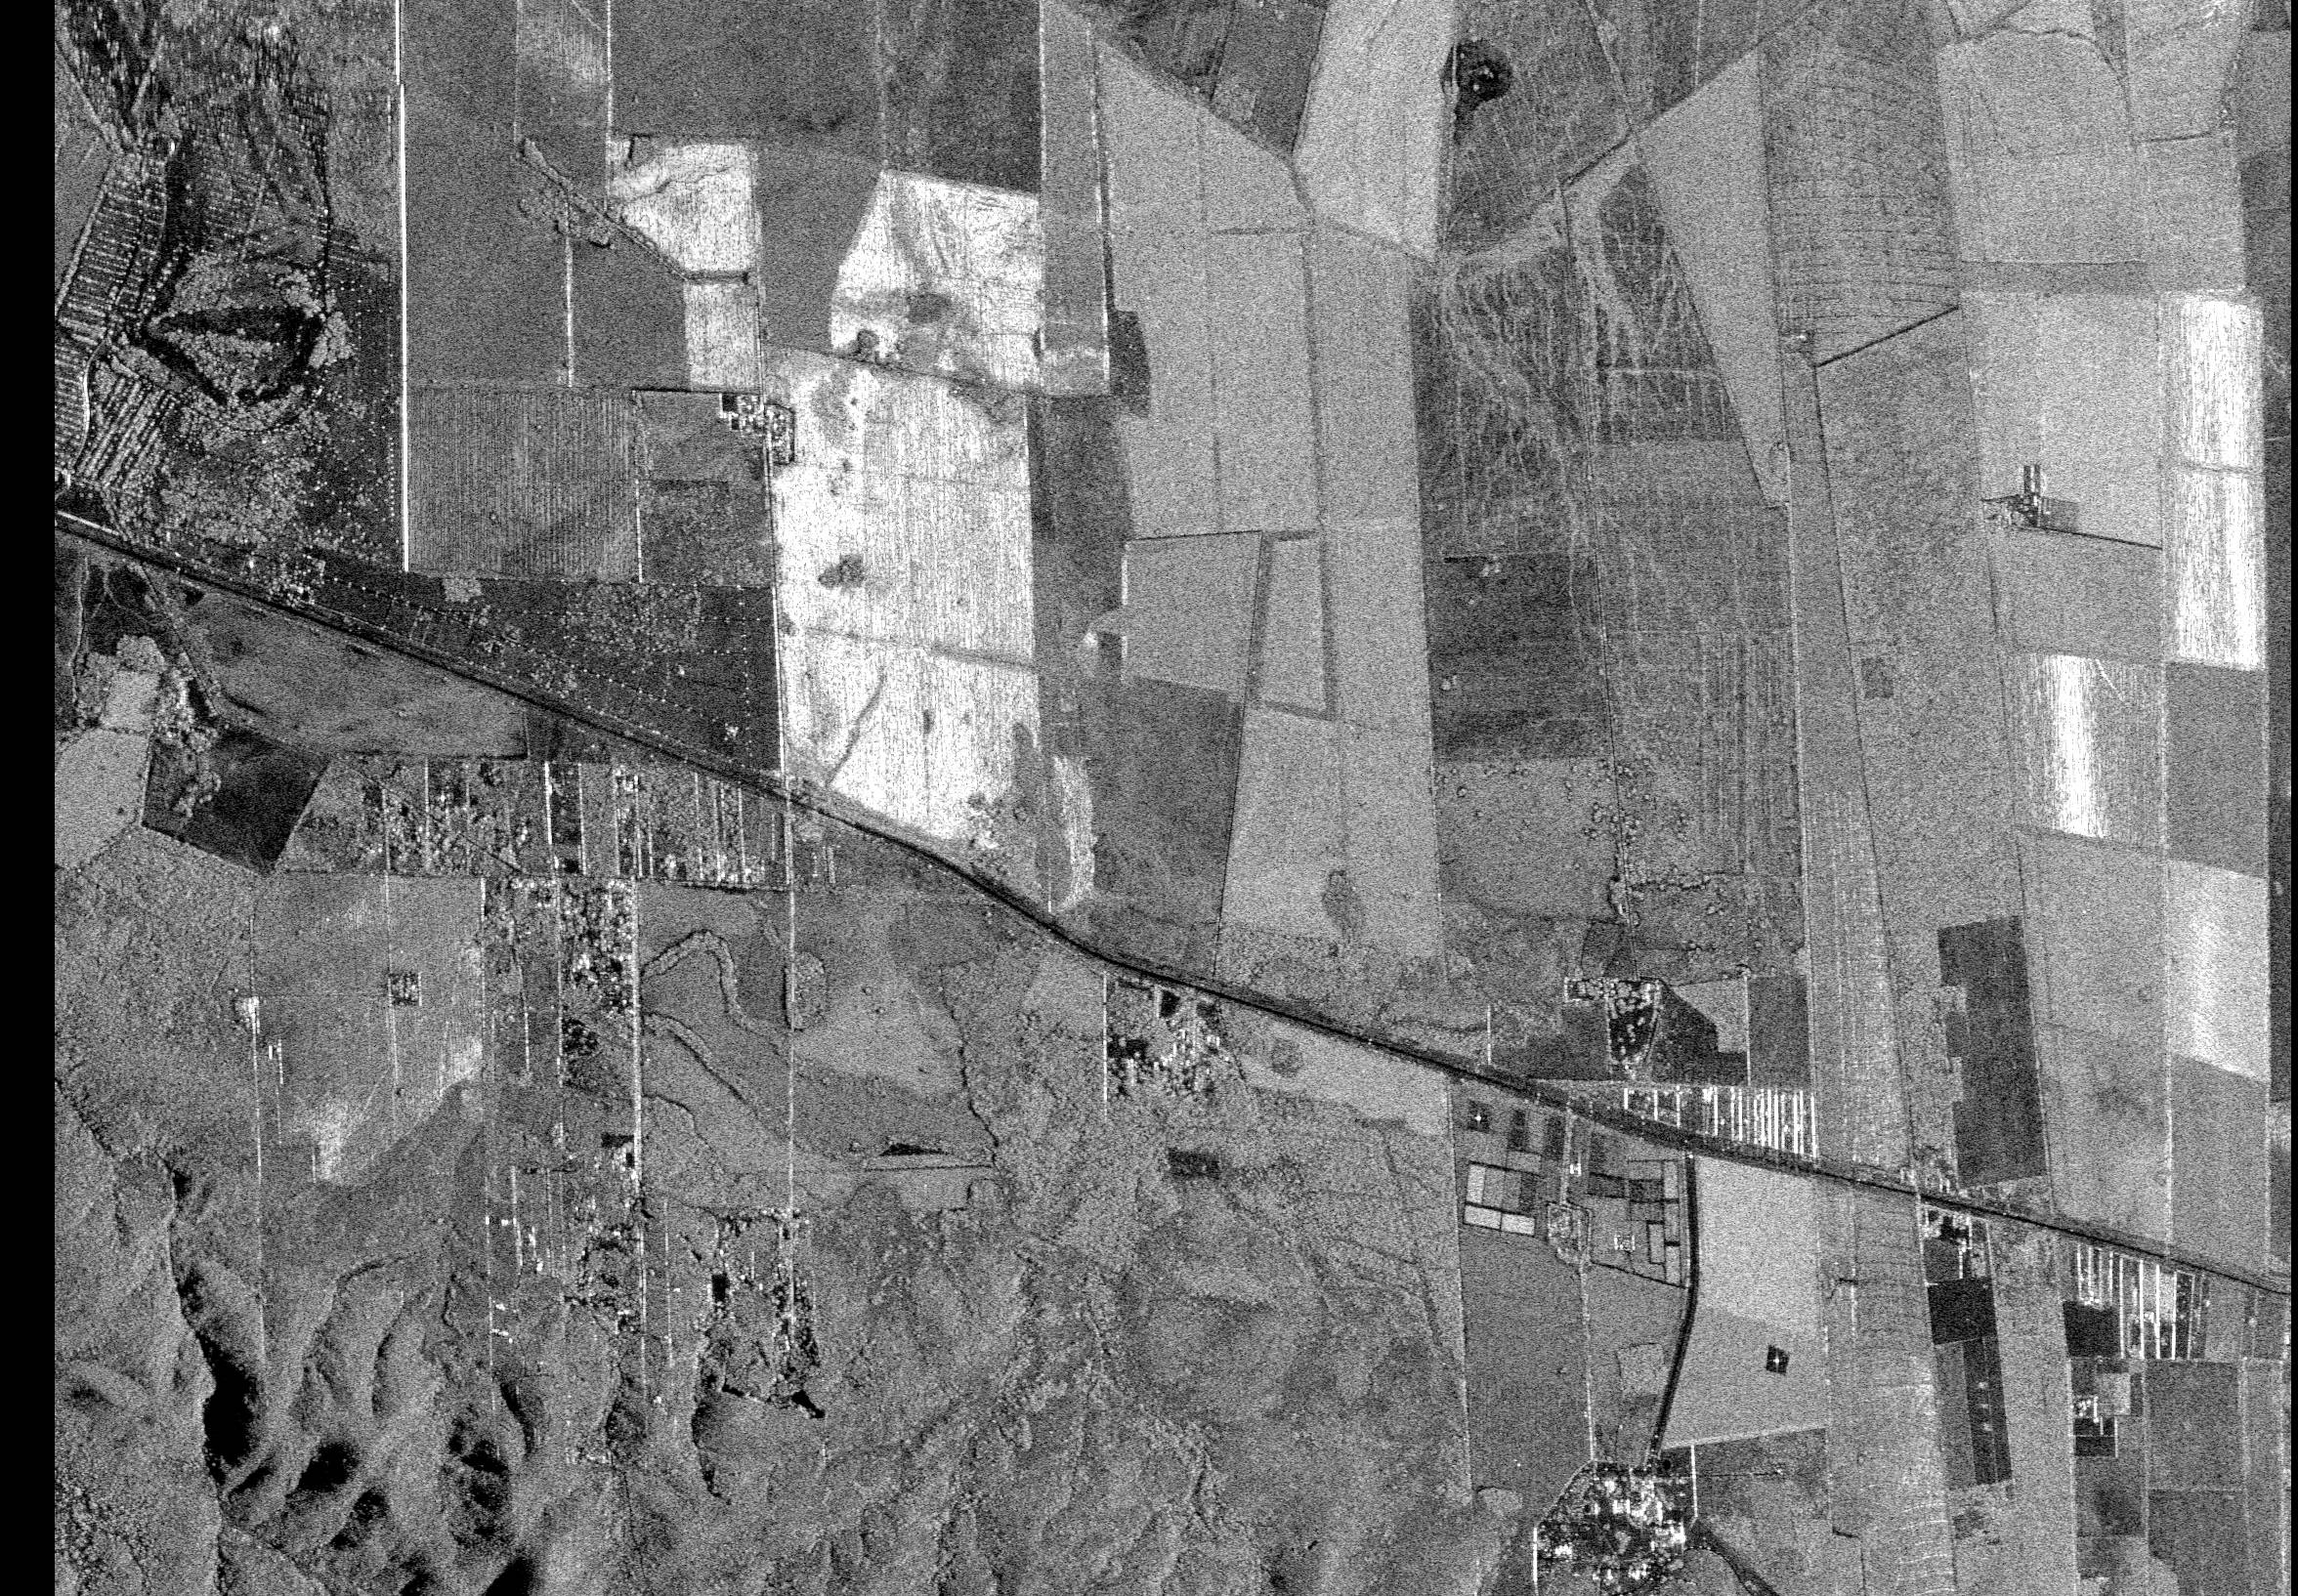
\includegraphics[height=0.2\textwidth]{fig:ground.jpg}
          \caption{}
          \label{}
        \end{figure}
    \end{column}
    \end{columns}
\end{frame}
%--- Next Frame --- %

\subsection{Niveles de procesamiento}
\begin{frame}{\secname : \subsecname}
  % Please add the following required packages to your document preamble:
  % \usepackage{booktabs}
  % \usepackage{graphicx}
  \begin{table}[]
  \centering
  \resizebox{\textwidth}{!}{%
  \begin{tabular}{@{}cccc@{}}
  \toprule
  L1A (SLC)                                                                                                    & L1B (GRD)                                                                  & L1C (GEC)                                                                              & L1D (GTC)                                                                                     \\ \midrule
  Single Look Complex                                                                                          & Ground Range Detected                                                      & Geocoded Elipsoid Corrected                                                            & Geocoded Terrain Corrected                                                                    \\
  \multicolumn{1}{p{4.5cm}}{Datos en formato complejo (real e imaginario), sin multilook y en la geometria del radar} & \multicolumn{1}{p{4.5cm}}{Datos en potencia, con multilook y proyectada al suelo} & \multicolumn{1}{p{4.5cm}}{Datos en potencia, con multilook y geocodificada sobe el elipsoide} & \multicolumn{1}{p{4.5cm}}{Datos en potencia, con multilook y geocodificada sobe el el terreno (DEM)}
  \end{tabular}%
  }
  \caption{Niveles de procesamiento típicos para una imagen SAR.}
  \label{my-label}
  \end{table}
\end{frame}
